\documentclass[11pt]{article}

\usepackage{theme}
\usepackage{shortcuts}
\usepackage{subcaption}
\usepackage{booktabs}
\usepackage{multirow}
\graphicspath{{figures/}{../figures/}} % figures/ inside the Overleaf zip, ../figures/ locally

% compact layout: the body must fit in 5 pages
\setlength{\parskip}{3pt}
\captionsetup{font=small}
\newcommand{\todo}[1]{\textcolor{red}{[TODO: #1]}}
\providecommand{\R}{\mathbb{R}}
\newcommand{\sdtw}{\mathrm{dtw}_\gamma}
\newcommand{\minop}{\mathop{\mathrm{min}^\gamma}}

\title{Soft-DTW, a Differentiable Loss Function for Time-Series}
\author{Pablo Borrego \email{pabloalmendralejo@gmail.com} \\ Pol Tibau \email{tibaurubaupol@gmail.com}}
\date{}

\begin{document}
\maketitle
\vspace{-1.5em}

% ======================================================================
\section{Introduction and contributions}


A time series can be defined as a matrix of the form $x=(x_1,\dots,x_n)\in\R^{n\times p}$, i.e.\ a sequence of $n$ observations $x_i\in\R^p$ ordered in time. So, given two time series $x\in\R^{n\times p}$ and $y\in\R^{m\times p}$, a fundamental problem arises: how can we work with them jointly if they have different supports? This is where DTW comes into play. DTW~\cite{sakoe1978dynamic} is a method that compares two series by first finding the cheapest monotone alignment between their time steps, so that shifts, local stretches and different lengths are not counted as differences; it is computed by dynamic programming in $O(nm)$ time. However, this method has some flaws, the biggest one being that it is not differentiable; therefore, it is not easy to use in a machine learning context. That is why Cuturi and Blondel~\cite{cuturi2017soft} introduced soft-DTW, a differentiable version of DTW with the same cost as DTW and with a gradient that allows us to apply ML tools. The paper uses it to compute barycenters, run $k$-means, classify with nearest centroids and train networks that output time series. 


\paragraph{Contributions and work repartition.}
\textbf{Implementation:} we implemented soft-DTW from scratch (forward and backward recursions in Numba, a PyTorch loss with the hand-written backward, and an anti-diagonal PyTorch version that runs on GPU).
\textbf{Reproduction:} we reproduce, on 10--13 UCR datasets, the paper's barycenter (Table 1), $k$-means (Table 2), nearest-centroid (Fig.~7) and forecasting (Table 3) experiments.
\textbf{Beyond the paper:} (i) we report magnitudes and computational costs that the paper omits; (ii) we propose soft-DTW with a warping penalty, which charges a cost $\omega$ for every time-stretching step (a soft version of amerced DTW~\cite{herrmann2023amercing}, computed as a soft dynamic program with step costs~\cite{mensch2018differentiable}); (iii) we compare it with soft-DTW in all four experiments of the paper (barycenters, $k$-means, nearest centroid and forecasting), with the paper's own protocols.
\textbf{Work repartition:} \todo{Discutir con Pol}.

% ======================================================================
\section{Method}

Let $x\in\R^{n\times p}$ and $y\in\R^{m\times p}$ be two time series. Matching $x_i$ with $y_j$ costs $\delta_{i,j}=\|x_i-y_j\|^2$, and these costs form the matrix $\Delta(x,y)=[\delta_{i,j}]_{i,j}\in\R^{n\times m}$. An \emph{alignment} is a path in this matrix from cell $(1,1)$ to cell $(n,m)$ made of three kinds of steps: $\searrow$ (both series advance), $\downarrow$ ($x$ advances while $y$ stays at the same point $y_j$) and $\rightarrow$ ($y$ advances while $x$ stays at $x_i$). We encode it as a binary matrix $A\in\{0,1\}^{n\times m}$, with $A_{i,j}=1$ if the path visits cell $(i,j)$, and write $\mathcal A_{n,m}$ for the set of all alignments. The cost of an alignment is the sum of the costs of the cells it visits, $\langle A,\Delta\rangle=\sum_{i,j}A_{i,j}\,\delta_{i,j}$, and DTW is the cost of the cheapest one:
\begin{equation}
\mathrm{dtw}(x,y)=\min_{A\in\mathcal A_{n,m}}\langle A,\Delta(x,y)\rangle .
\end{equation}

Soft-DTW replaces this minimum by the \emph{soft-minimum} with smoothing parameter $\gamma>0$,
\begin{equation}
\minop(a_1,\dots,a_k)=-\gamma\log\sum_{l=1}^{k}e^{-a_l/\gamma}.
\end{equation}
Therefore, soft-DTW is the soft-minimum of the costs of all alignments:
\begin{equation}
\sdtw(x,y)=\minop_{A\in\mathcal A_{n,m}}\langle A,\Delta(x,y)\rangle=-\gamma\log\sum_{A\in\mathcal A_{n,m}}e^{-\langle A,\Delta(x,y)\rangle/\gamma}.
\end{equation}
The soft-minimum tends to $\min(a_1,\dots,a_k)$ as $\gamma\to0$ (we write $\min^{0}=\min$), but unlike the minimum it is a smooth function of its arguments: its derivative with respect to $a_l$ is the softmax weight $e^{-a_l/\gamma}/\sum_{l'}e^{-a_{l'}/\gamma}\in(0,1)$, so the smallest values weigh most but all of them contribute. Hence $\sdtw$ is smooth (infinitely differentiable) in $\Delta$, and so in $x$, whereas $\mathrm{dtw}$ has kinks wherever the optimal path changes.
\paragraph{Forward pass (Algorithm 1).}
It is impossible to find the minimum by computing all the alignments, as $|\mathcal A_{n,m}|$ is a Delannoy number, which grows exponentially with $n$ and $m$; therefore, we need a dynamic programming approach. Both DTW and soft-DTW are computed by Bellman's recursion: with $r_{0,0}=0$ and $r_{i,0}=r_{0,j}=+\infty$,
\begin{equation}
r_{i,j}=\delta_{i,j}+\minop\{r_{i-1,j-1},\,r_{i-1,j},\,r_{i,j-1}\},\qquad \sdtw(x,y)=r_{n,m},
\end{equation}
in $O(nm)$ time.

We want to understand how much $r_{n,m}=\sdtw(x,y)$ changes if we change the series $x$; mathematically, this is expressed by the gradient $\nabla_x\sdtw(x,y)=\partial r_{n,m}/\partial x$. Since $x$ only enters the recursion through the costs $\delta_{i,j}$, and each $\delta_{i,j}$ is added to $r_{i,j}$ only, thanks to the chain rule we get
\begin{equation}
\nabla_x\sdtw(x,y)=\sum_{i,j}\frac{\partial r_{n,m}}{\partial \delta_{i,j}}\,\frac{\partial \delta_{i,j}}{\partial x}=\sum_{i,j}e_{i,j}\,\frac{\partial \delta_{i,j}}{\partial x},\qquad e_{i,j}:=\frac{\partial r_{n,m}}{\partial r_{i,j}} .
\end{equation}
This means that the gradient can be interpreted in terms of how much $r_{n,m}$ depends on each $r_{i,j}$ (the coefficient $e_{i,j}$) and of how much each cell depends on $x$, given by $\partial\delta_{i,j}/\partial x_i=2(x_i-y_j)$ (and $0$ for the other points $x_k$, $k\neq i$). In (3), each alignment $A$ enters with weight $e^{-\langle A,\Delta\rangle/\gamma}$, so cheap alignments weigh much more than expensive ones; normalised, these weights define a probability $p_\gamma(A)$ for each alignment. If we increase the cost $\delta_{i,j}$ of one cell slightly, only the alignments that pass through $(i,j)$ become more expensive, so soft-DTW increases in proportion to their share of the total weight. Hence $e_{i,j}=\partial r_{n,m}/\partial\delta_{i,j}$ is the probability that an alignment drawn from $p_\gamma$ passes through cell $(i,j)$, and $E=[e_{i,j}]$ is the \emph{expected alignment} $\mathbb E_\gamma[A]$. Computing this expectation naively costs $O(n^2m^2)$; instead, the paper back-propagates through the recursion. Since $r_{i,j}$ only influences its three successors,
\begin{equation}
e_{i,j}=\sum_{(k,l)\in\{(i+1,j),(i,j+1),(i+1,j+1)\}} e_{k,l}\,\exp\!\big((r_{k,l}-r_{i,j}-\delta_{k,l})/\gamma\big),\qquad e_{n,m}=1,
\end{equation}
where each exponential is the softmax weight of $r_{i,j}$ inside $r_{k,l}$, and can be read directly from the table $R=[r_{i,j}]$ computed in the forward pass, which is therefore kept in memory. As $\gamma\to0$, $E$ tends to the optimal DTW path $A^\star$, whose discontinuous dependence on $x$ is what soft-DTW removes (Fig.~\ref{fig:E}).

These algorithms provide the tools to find a minimum of soft-DTW; note that this is only a local minimum, as the problem is not convex. We can use soft-DTW as a loss (or error) function to compute different objects from a set of time series, such as averages, clusters, classifiers or forecasts. The most popular one is the barycenter (average) of a set of series $y_1,\dots,y_N$, which is computed as the series $x$ that solves $\min_x\sum_i \frac{\lambda_i}{m_i}\sdtw(x,y_i)$; we find it with L-BFGS.

In the recursion above, the three steps that can enter cell $(i,j)$ all cost the same $\delta_{i,j}$, which means that stretching time is free in soft-DTW. We propose to charge a fixed penalty $\omega\ge0$ for every step that stretches time ($\downarrow$ and $\rightarrow$), while the diagonal step $\searrow$ keeps its cost:
\begin{equation}
r_{i,j}=\minop\{r_{i-1,j-1}+\delta_{i,j},\; r_{i-1,j}+\delta_{i,j}+\omega,\; r_{i,j-1}+\delta_{i,j}+\omega\}.
\end{equation}
We call it soft-DTW$_\omega$. Forward and backward passes are unchanged, so the gradient is computed as before. The motivation is that soft-DTW has a built-in preference: for large $\gamma$, $E$ concentrates around the diagonal whatever the data (Fig.~\ref{fig:E}, right), and the penalty is a way to control how much warping is allowed (Fig.~\ref{fig:prior} in the appendix).

% ======================================================================
\section{Data}
\label{sec:data}

We use 13 univariate datasets of the UCR archive~\cite{ucr2018} (loaded with \texttt{tslearn}~\cite{tavenard2020tslearn}, which we also use for the DBA baseline and as a numerical cross-check), chosen to span domains (ECG, motion, image outlines, power demand, synthetic), lengths (24 to 512) and numbers of classes (2 to 60), while keeping the quadratic cost of DTW manageable on a laptop (Table~\ref{tab:data}). The paper used a subset of 79 datasets without stating the selection criterion.

All series are z-normalised (mean 0, standard deviation 1 per series), as provided by the UCR archives, so pointwise costs $\delta_{i,j}$ are $O(1)$. To check whether the data actually contain the temporal distortions DTW is designed for, we drew 200 random pairs of series of the same class per dataset and measured (i) the global lag maximising their cross-correlation and (ii) the fraction of the Euclidean cost removed by DTW, $1-\mathrm{dtw}/\|x-y\|^2$. Two regimes appear. Datasets such as CBF, Trace, SyntheticControl or ECG200 contain large global shifts (10\% of the pairs are shifted by 15--35\% of the length). Others (Coffee, ArrowHead, Plane) are globally aligned (lag $0$), yet DTW still removes 68--90\% of the Euclidean cost: the variability is made of \emph{local} accelerations and stretches, which a global shift cannot fix but warping can. In every dataset DTW removes between 48\% and 96\% of the within-class Euclidean cost, which supports using an elastic geometry on all of them.

\begin{table}[t]
\centering\small
\caption{Datasets and diagnosis, over 200 random pairs $(x,y)$. Lag $=\frac{100}{n}\big|\arg\max_k \sum_t (x_t-\bar x)(y_{t+k}-\bar y)\big|$. Interpreted as the shift that best superimposes the two series (cross-correlation), in \% of the length $n$; median / 90th percentile over the pairs. DTW gain $=1-\mathrm{dtw}(x,y)/|x-y|^2$.}
\label{tab:data}
\begin{tabular}{lrrrrcc}
\toprule
Dataset & Train & Test & Length & Classes & Lag \% (med / p90) & DTW gain \\
\midrule
ItalyPowerDemand & 67 & 1029 & 24 & 2 & 0.0 / 8.3 & 0.48 \\
SyntheticControl & 300 & 300 & 60 & 6 & 3.3 / 35.2 & 0.76 \\
TwoLeadECG & 23 & 1139 & 82 & 2 & 2.4 / 6.1 & 0.90 \\
ECG200 & 100 & 100 & 96 & 2 & 2.1 / 19.8 & 0.79 \\
MedicalImages & 381 & 760 & 99 & 10 & 1.0 / 8.2 & 0.78 \\
CBF & 30 & 900 & 128 & 3 & 4.7 / 25.8 & 0.85 \\
ECGFiveDays & 23 & 861 & 136 & 2 & 1.5 / 3.7 & 0.90 \\
Plane & 105 & 105 & 144 & 7 & 0.0 / 0.7 & 0.90 \\
GunPoint & 50 & 150 & 150 & 2 & 0.7 / 5.3 & 0.77 \\
ArrowHead & 36 & 175 & 251 & 3 & 0.0 / 0.0 & 0.85 \\
Trace & 100 & 100 & 275 & 4 & 4.7 / 14.6 & 0.96 \\
Coffee & 28 & 28 & 286 & 2 & 0.0 / 0.0 & 0.68 \\
ShapesAll & 600 & 600 & 512 & 60 & 1.2 / 27.1 & 0.93 \\
\bottomrule
\end{tabular}
\end{table}

% ======================================================================
\section{Results}

\subsection{Implementation and verification}
Forward and backward passes are compiled with Numba, with the soft-minimum computed in a numerically stable way (log-sum-exp trick); a PyTorch \texttt{autograd.Function} calls them, and a second, pure PyTorch version processes whole anti-diagonals at once ($n+m$ sequential steps instead of $nm$). We check the soft-DTW value $r_{n,m}$ (Algorithm 1) and the expected alignment $E$ (Algorithm 2) against \emph{brute-force enumeration of every alignment} (all Delannoy paths, $n,m\le5$, $\gamma\in[10^{-2},10]$, error $<10^{-10}$), the gradient against finite differences, the bound $\mathrm{dtw}-\gamma\log|\mathcal A|\le\sdtw\le\mathrm{dtw}$, the agreement with \texttt{tslearn}, and the custom backward against autograd. All variants scale as $O(nm)$ (fitted log-log slopes $2.02$--$2.04$), but constants differ by orders of magnitude: for $n=m=64$ forward+backward takes $0.3$\,ms with Numba, $20$\,ms with the same code in pure Python and $0.75$\,s with a cell-by-cell PyTorch forward differentiated by autograd, which confirms the paper's remark that a custom backward is essential.

\subsection{Barycenters and $k$-means}
Protocol as in the paper: for each dataset, 10 random draws of 10 series of one class; barycenters from the same initialisation (random $\mathcal N(0,1)$ or Euclidean mean) with at most 100 iterations; soft-DTW with L-BFGS, DBA~\cite{petitjean2011global} (\texttt{tslearn}) and a batch subgradient method with backtracking line search~\cite{schultz2018nonsmooth}. All methods are scored with the \emph{hard} DTW objective (Eq.~4 with $\gamma=0$), which is the objective DBA itself minimises. $k$-means uses $k$ = number of classes, at most 30 Lloyd and 100 barycenter iterations, training sets capped at 100 series, 3 random initialisations (random series) and a Euclidean $k$-means initialisation.

\begin{table}[t]
\centering\small
\caption{Percentage of datasets on which soft-DTW (resp.\ soft-DTW$_\omega$) reaches a lower hard-DTW loss than DBA / the subgradient method. Ours (12 datasets for barycenters, 10 for $k$-means) vs.\ the paper (79 datasets) in parentheses. Soft-DTW$_\omega$ uses the same draws and initialisations, with $\omega=0.1$ (left of the slash) and $\omega=1$ (right).}
\label{tab:repro}
\setlength{\tabcolsep}{3pt}
\begin{tabular}{lllcccc}
\toprule
& Method & Compared with & $\gamma=1$ & $\gamma=0.1$ & $\gamma=0.01$ & $\gamma=0.001$ \\
\midrule
\multirow{8}{*}{\rotatebox{90}{Barycenters}}
& \multirow{4}{*}{soft-DTW} & DBA, random init & 58 (41) & 92 (94) & 100 (100) & 100 (97) \\
& & DBA, Euclidean init & 8 (4) & 25 (47) & 75 (80) & 100 (90) \\
& & subgrad., random init & 75 (96) & 100 (97) & 100 (97) & 100 (97) \\
& & subgrad., Euclidean init & 17 (35) & 75 (72) & 92 (92) & 100 (97) \\
\cmidrule{2-7}
& \multirow{4}{*}{\shortstack[l]{soft-DTW$_\omega$\\{\scriptsize $\omega=0.1$ / $\omega=1$}}} & DBA, random init & 58 / 58 & 83 / 58 & 83 / 58 & 83 / 58 \\
& & DBA, Euclidean init & 8 / 8 & 17 / 8 & 8 / 8 & 8 / 8 \\
& & subgrad., random init & 75 / 83 & 100 / 100 & 100 / 100 & 100 / 100 \\
& & subgrad., Euclidean init & 17 / 17 & 50 / 17 & 58 / 17 & 58 / 17 \\
\midrule
\multirow{8}{*}{\rotatebox{90}{$k$-means}}
& \multirow{4}{*}{soft-DTW} & DBA, random init & 10 (16) & 50 (25) & 70 (60) & 90 (77) \\
& & DBA, Euclidean init & 10 (29) & 10 (24) & 60 (55) & 90 (69) \\
& & subgrad., random init & 20 (42) & 60 (58) & 100 (76) & 90 (96) \\
& & subgrad., Euclidean init & 10 (46) & 10 (50) & 90 (66) & 100 (84) \\
\cmidrule{2-7}
& \multirow{4}{*}{\shortstack[l]{soft-DTW$_\omega$\\{\scriptsize $\omega=0.1$ / $\omega=1$}}} & DBA, random init & 10 / 10 & 40 / 10 & 40 / 20 & 40 / 20 \\
& & DBA, Euclidean init & 10 / 0 & 10 / 0 & 10 / 0 & 20 / 0 \\
& & subgrad., random init & 20 / 20 & 70 / 30 & 60 / 30 & 60 / 30 \\
& & subgrad., Euclidean init & 10 / 0 & 20 / 0 & 10 / 0 & 20 / 0 \\
\bottomrule
\end{tabular}
\end{table}

Table~\ref{tab:repro} reproduces the paper's benchmark for barycenters and $k$-means and also adds soft-DTW$_\omega$ to the comparison. For soft-DTW we obtain results similar to the paper's: small $\gamma$ beats DBA almost always, $\gamma=1$ rarely does, and the gap is larger from a random start. For barycenters with a random start the median soft-DTW/DBA loss ratio is $0.86$ ($\gamma=0.01$), down to $0.26$ on Plane ($\gamma=0.1$), where DBA is trapped in a poor local minimum; from the Euclidean mean, which is already a good start, the gain is only $3$--$4\%$ (median ratio $0.97$). For $k$-means the gains shrink further (median ratio $0.97$ for $\gamma\le0.01$). As for the cost, with $\gamma=0.001$ a soft-DTW barycenter takes $14\times$ (and a $k$-means run $16\times$) the time of DBA, because the objective becomes nearly non-smooth and L-BFGS needs many more steps. Conversely, $\gamma=1$ gives visually smooth barycenters and centroids, as in the paper's qualitative figures, which we reproduce in the appendix (Figs.~\ref{fig:bary}--\ref{fig:kmeans}), but losses up to $3\times$ that of DBA, mainly because smoothness and fidelity to DTW pull in opposite directions, and the hard-DTW metric only rewards the latter. Finally, the subgradient baseline is very sensitive to its step size, which inflates the win rates against it.

Our soft-DTW$_\omega$ outperforms soft-DTW from a random start: with $\gamma=\omega=0.1$ its barycenters have an $8\%$ lower DTW loss than soft-DTW ($\gamma=0.01$) and are computed $1.3\times$ faster, since the penalty removes many degenerate paths from the soft-minimum. It beats DBA on fewer datasets than soft-DTW, but by more where DBA is trapped (down to $0.21\times$ its loss). From the Euclidean mean and in $k$-means, plain soft-DTW remains best. Decreasing $\gamma$ brings soft-DTW closer to the DTW loss used for scoring, so its win rate against DBA rises to 100\%; soft-DTW$_\omega$ instead gets closer to DTW plus a warping penalty, a different objective, so its win rate does not improve.

\subsection{Nearest-centroid classification}
We can also use the barycenter to classify series. Each class is represented by the barycenter of its training series (its centroid), and every new series is given the class of the closest centroid. The paper uses this to compare soft-DTW and DBA barycenters; we add soft-DTW$_\omega$.

As in the paper, we merge the train and test sets of each dataset and split them randomly into train (50\%), validation (25\%) and test (25\%), three times. Centroids are computed on the train part, starting from the Euclidean mean of each class. Each method uses its own distance to find the closest centroid: hard DTW for DBA, $\sdtw$ for soft-DTW and soft-DTW$_\omega$ for soft-DTW$_\omega$. The parameters $\gamma$ (15 values between $10^{-3}$ and $10$) and $\omega\in\{0.1,1\}$ are chosen on the validation part.

The key insight is that soft-DTW centroids classify better than DBA centroids: they are at least as accurate on 83\% of the datasets (paper: 75\%). Soft-DTW$_\omega$ does not improve on soft-DTW: it is better on 6 datasets and worse on 4.

\subsection{Multistep-ahead forecasting}
Soft-DTW can also be used as a training loss. Following the paper, we train a network to forecast the end of a series: it sees the first 60\% of the series and must predict the remaining 40\%. The network is an MLP (one hidden layer of 256 sigmoid units, trained with Adam for 400 epochs; the paper does not give these values). We train it with three losses: the Euclidean loss, soft-DTW and our soft-DTW$_\omega$. The soft-DTW and soft-DTW$_\omega$ networks are trained in two ways: from scratch (random weights), or by taking the network already trained with the Euclidean loss and continuing its training with soft-DTW (resp.\ soft-DTW$_\omega$). We use 13 datasets.

Once trained, each network forecasts the test series, and we measure the error of these forecasts in two ways: with DTW, which forgives small shifts in time, and with the Euclidean distance, which does not. On each dataset we rank the losses from best (1) to worst, and Table~\ref{tab:forecast} gives the average rank over the 13 datasets, next to the paper's values.

\begin{table}[h]
\centering\small
\caption{Average rank (1 = best) of each training loss on the test forecasts, over 13 datasets; the paper's values (79 datasets) in parentheses. Rows soft-DTW$_\omega$: rank of soft-DTW$_\omega$ with $\omega=0.1$ (left of the slash) and $\omega=1$ (right) when it replaces soft-DTW with the same $\gamma$.}
\label{tab:forecast}
\setlength{\tabcolsep}{2.6pt}
\begin{tabular}{lllccccc}
\toprule
Metric & Init & & Euclidean & $\gamma=1$ & $\gamma=0.1$ & $\gamma=0.01$ & $\gamma=0.001$ \\
\midrule
\multirow{4}{*}{DTW} & \multirow{2}{*}{random} & soft-DTW & 3.69 (3.46) & 3.92 (3.55) & 2.31 (3.33) & 2.23 (2.79) & 2.85 (1.87) \\
& & soft-DTW$_\omega$ ($\omega=0.1$ / $1$) & & 3.92 / 3.92 & 2.15 / 3.00 & 2.08 / 3.31 & 2.08 / 3.38 \\
& \multirow{2}{*}{Euclidean} & soft-DTW & 3.92 (4.21) & 4.46 (3.96) & 2.85 (3.42) & 2.08 (2.12) & 1.69 (1.29) \\
& & soft-DTW$_\omega$ ($\omega=0.1$ / $1$) & & 4.46 / 4.08 & 2.46 / 3.15 & 2.38 / 2.92 & 2.46 / 2.92 \\
\midrule
\multirow{4}{*}{Euclidean} & \multirow{2}{*}{random} & soft-DTW & 1.31 (1.05) & 1.69 (2.41) & 3.46 (3.42) & 4.00 (4.13) & 4.54 (3.99) \\
& & soft-DTW$_\omega$ ($\omega=0.1$ / $1$) & & 1.69 / 1.77 & 3.31 / 2.00 & 3.15 / 1.92 & 3.23 / 1.85 \\
& \multirow{2}{*}{Euclidean} & soft-DTW & 2.77 (1.70) & 1.62 (2.99) & 2.38 (3.38) & 3.77 (3.64) & 4.46 (3.29) \\
& & soft-DTW$_\omega$ ($\omega=0.1$ / $1$) & & 1.62 / 1.69 & 2.23 / 2.38 & 2.77 / 2.38 & 2.62 / 2.23 \\
\bottomrule
\end{tabular}
\end{table}

As in the paper, when the forecasts are evaluated with DTW, the networks trained with soft-DTW and a small $\gamma$ rank best, whereas with the Euclidean distance the network trained with the Euclidean loss does. Moreover, when training starts from the Euclidean network, the smaller $\gamma$, the better the DTW rank: for $\gamma\le0.01$ the median test DTW is $19$--$20\%$ lower than that of the Euclidean network.

We also find two differences with the paper. First, with $\gamma=0.001$ and random weights, training is unstable on some datasets: on Coffee the test DTW is $3.2\times$ that of the Euclidean network, as also reported in~\cite{zeitler2023stabilizing}, and starting from the Euclidean network removes the problem. Second, ignoring time has a high price: soft-DTW forecasts have the right shape but at the wrong place, so their Euclidean error is $1.5\times$ ($\gamma=0.1$) to $3.4\times$ ($\gamma=0.001$) that of the Euclidean network.

Beyond these differences, Fig.~\ref{fig:forecast} shows a more serious failure. On ShapesAll, the network trained with soft-DTW predicts an almost flat line with a few isolated spikes, and yet its test DTW is \emph{lower} than that of the Euclidean network ($6.6$ vs.\ $9.3$). The reason is that DTW can match a single point of the prediction with a whole segment of the true series: one spike at the right height is enough to ``cover'' an entire rise. Such predictions are therefore cheap for DTW, both when training and when evaluating. Soft-DTW does not penalise these stretchings~\cite{leguen2019shape}; soft-DTW$_\omega$ does, by charging $\omega$ for each of them.

\begin{figure}[t]
\centering
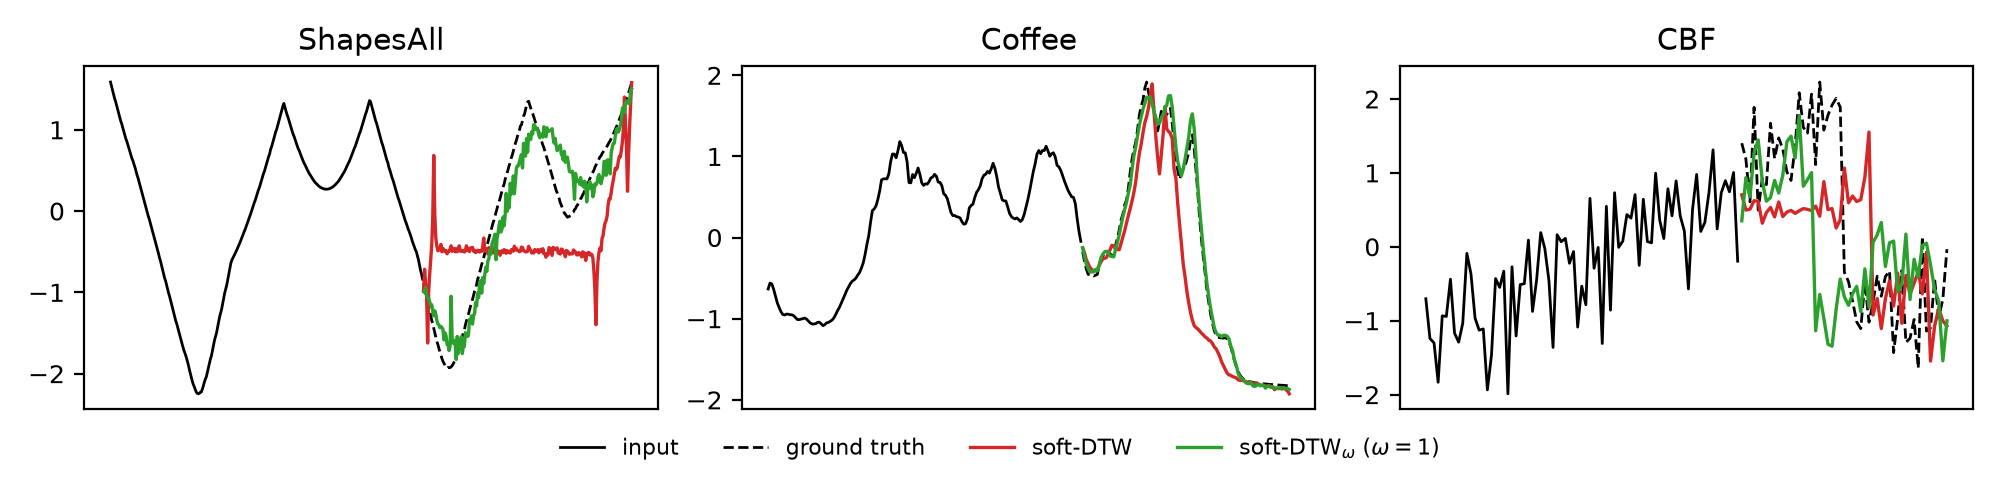
\includegraphics[width=\linewidth]{forecast_omega_examples.png}
\caption{Test forecasts (last 40\%) of networks trained from random weights with soft-DTW and with soft-DTW$_\omega$ ($\omega=1$), $\gamma=0.01$. On ShapesAll soft-DTW degenerates into a flat line with spikes, which DTW scores better than the Euclidean forecast; the warping penalty removes it.}
\label{fig:forecast}
\end{figure}

The soft-DTW$_\omega$ rows of Table~\ref{tab:forecast} show the effect of this penalty. From random weights, a small penalty ($\omega=0.1$) is almost free: it improves the DTW rank of soft-DTW for every $\gamma\le0.1$, and for $\gamma\le0.01$ it also lowers the Euclidean error by $30\%$. A larger penalty ($\omega=1$) loses $6$--$9\%$ in DTW but divides the Euclidean error by $2$ to $3$, on all 13 datasets, which brings its Euclidean rank close to that of the Euclidean network. The penalty also removes the failures described above: on ShapesAll the flat line with spikes disappears (Fig.~\ref{fig:forecast}), and with $\gamma=0.001$ the unstable runs are fixed (test DTW $1.44\to0.44$ on Coffee and $0.69\to0.35$ on Plane, $\omega=1$). From the Euclidean network, which already avoids these failures, the effect is small.

% ======================================================================
\section{Conclusion}
We re-implemented soft-DTW from scratch, verified it against exhaustive enumeration of alignments, and reproduced the paper's four experiments (barycenters, $k$-means, nearest centroid and forecasting) on 10--13 UCR datasets: the main claims hold, as do the trends in $\gamma$. Measuring magnitudes and costs shows their limits: large gains over DBA only from poor initialisations, and a 10--15$\times$ computational overhead for the small $\gamma$ that win. In forecasting, the free warping of soft-DTW leads to unstable training and degenerate predictions that DTW itself scores well. Charging a penalty $\omega$ for each time-stretching step fixes these failures and gives a controllable trade-off between shape and timing. It also improves barycenters from poor initialisations, but not from a good one, and it does not improve $k$-means or nearest-centroid classification.


\bibliographystyle{plain}
\bibliography{bib}

\appendix
% ======================================================================
\section{Additional figures}

\begin{figure}[h]
\centering
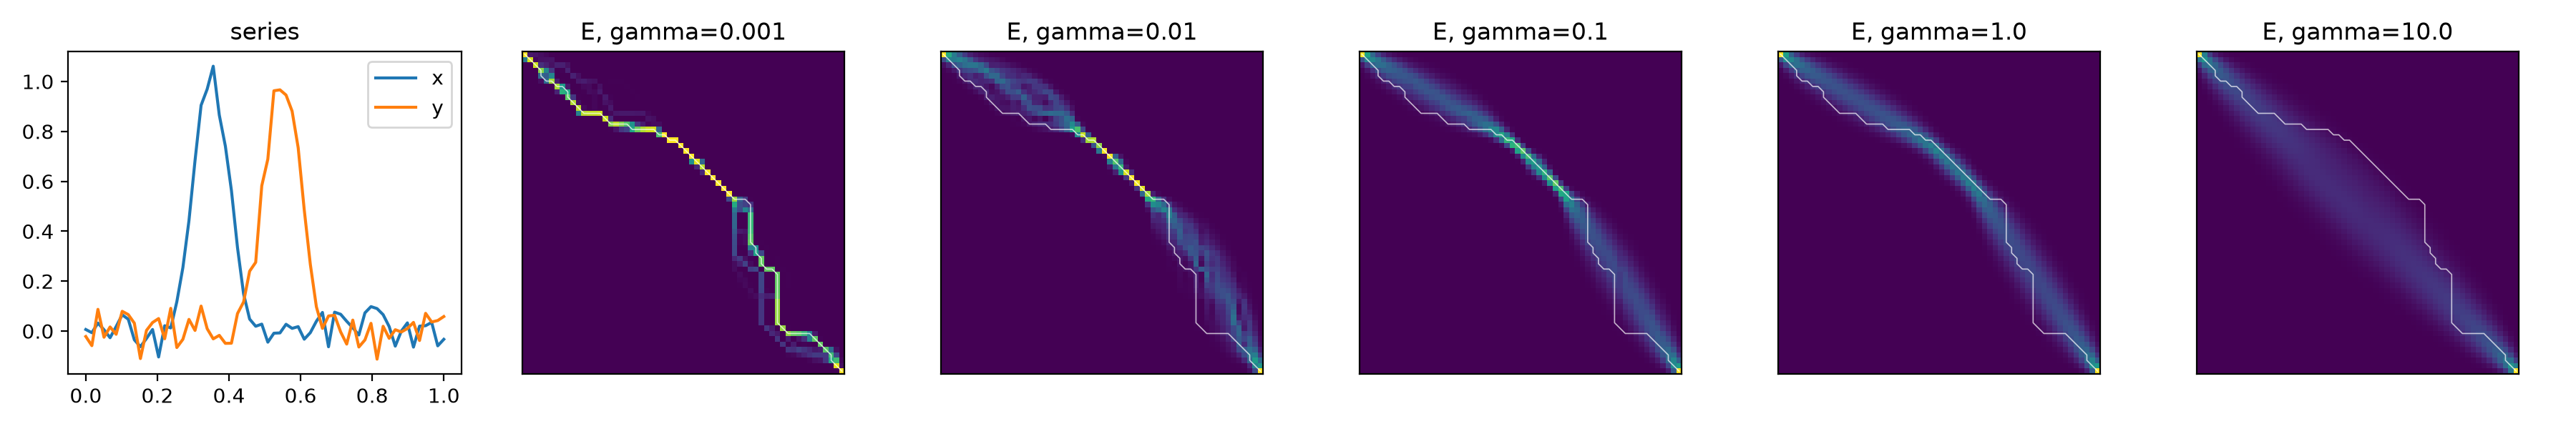
\includegraphics[width=\linewidth]{E_vs_gamma.png}
\caption{Expected alignment $E=\mathbb E_\gamma[A]$ between two shifted bumps for increasing $\gamma$; white: optimal DTW path. For $\gamma=10$ the alignment ignores the data and concentrates around the diagonal.}
\label{fig:E}
\end{figure}

\begin{figure}[h]
\centering
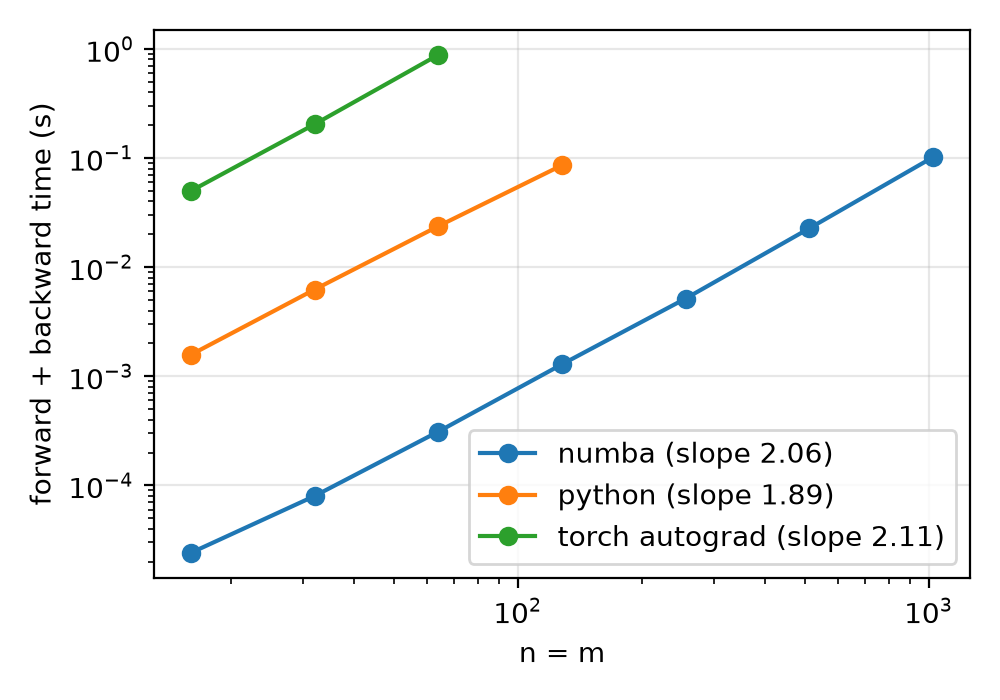
\includegraphics[width=0.55\linewidth]{timing.png}
\caption{Forward + backward time vs.\ length $n=m$ (log-log). All implementations are quadratic; Numba is $\sim$65$\times$ faster than the same code in pure Python and $\sim$2400$\times$ faster than a cell-by-cell PyTorch forward differentiated by autograd ($n=64$).}
\label{fig:timing}
\end{figure}

\begin{figure}[h]
\centering
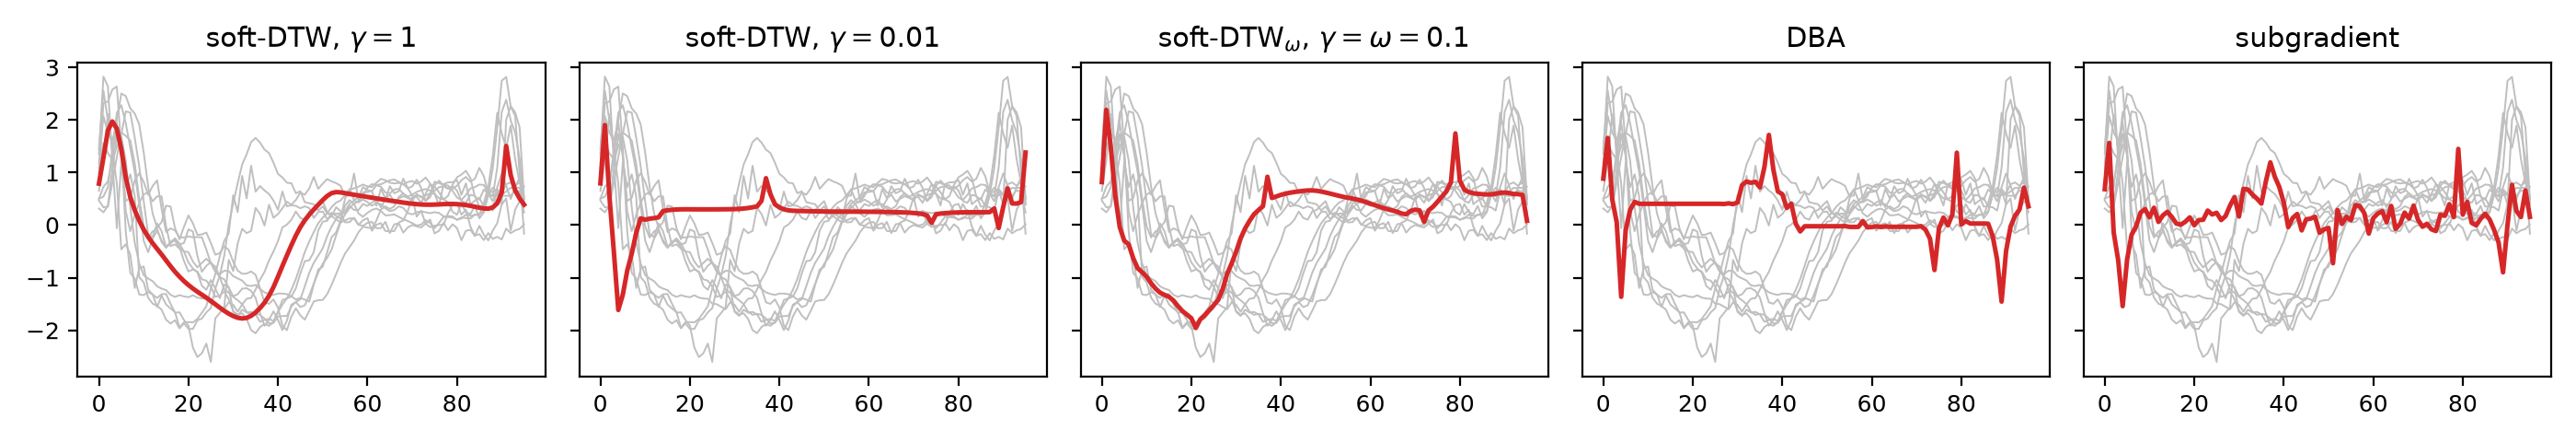
\includegraphics[width=\linewidth]{barycenters_ECG200.png}
\caption{Barycenters of 10 ECG200 series (grey) from the same random initialisation (paper's Fig.~5). With $\gamma=1$ the barycenter is smooth and follows the shape of the class; with $\gamma=0.01$, DBA and the subgradient method it shows spurious kinks and flat segments. Soft-DTW$_\omega$ ($\gamma=\omega=0.1$) recovers the valley of the class with little smoothing, keeping a few kinks.}
\label{fig:bary}
\end{figure}

\begin{figure}[h]
\centering
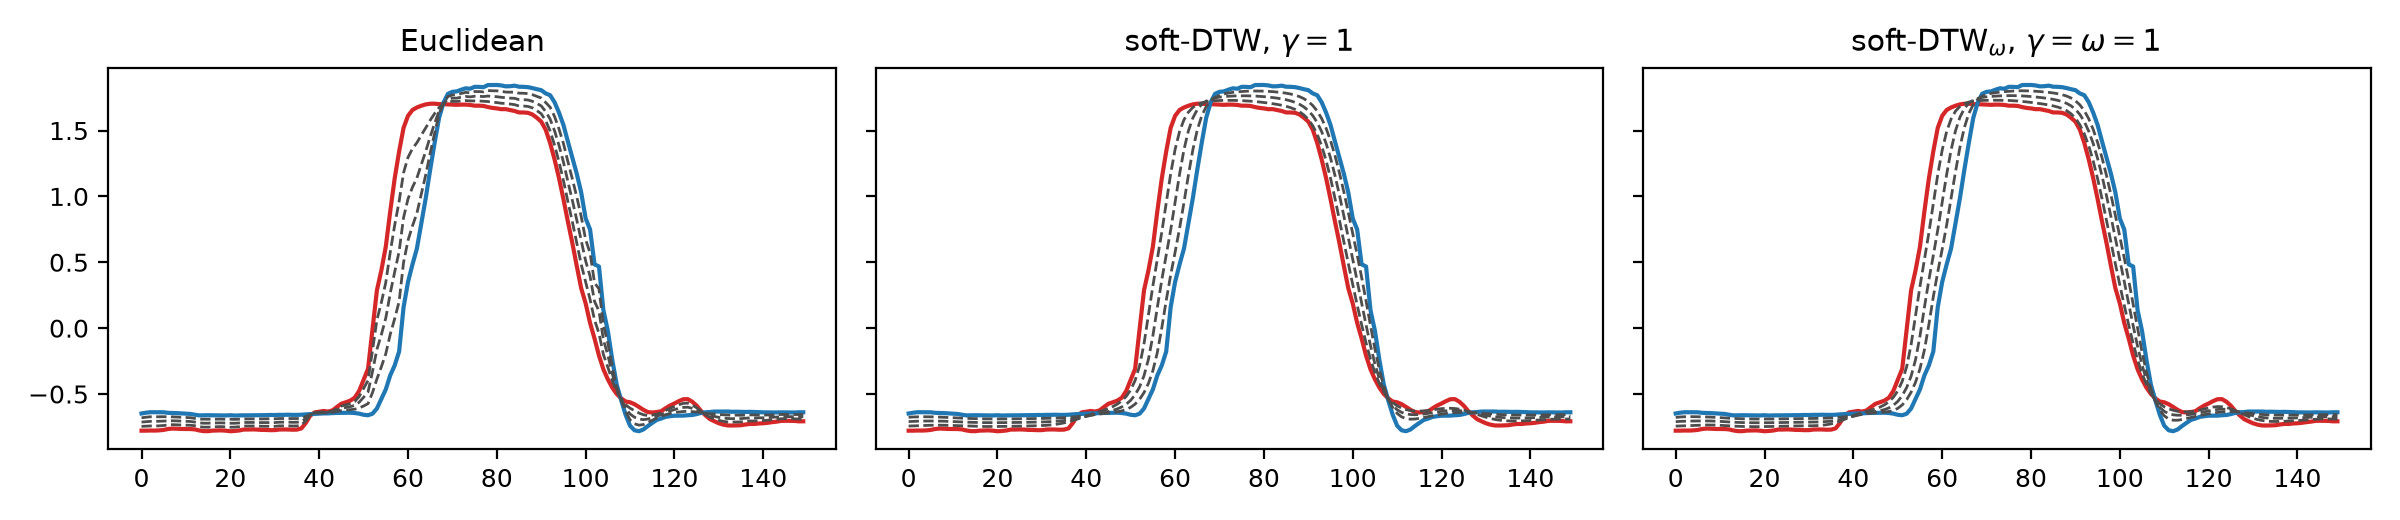
\includegraphics[width=0.8\linewidth]{interpolation_GunPoint.png}
\caption{Weighted barycenters (dashed, weights $0.25,0.5,0.75$) between two GunPoint series (paper's Fig.~4). The Euclidean average blends the two pulses, whereas soft-DTW moves the pulse in time from one series to the other; soft-DTW$_\omega$ ($\gamma=\omega=1$) gives almost the same interpolation.}
\label{fig:interp}
\end{figure}

\begin{figure}[h]
\centering
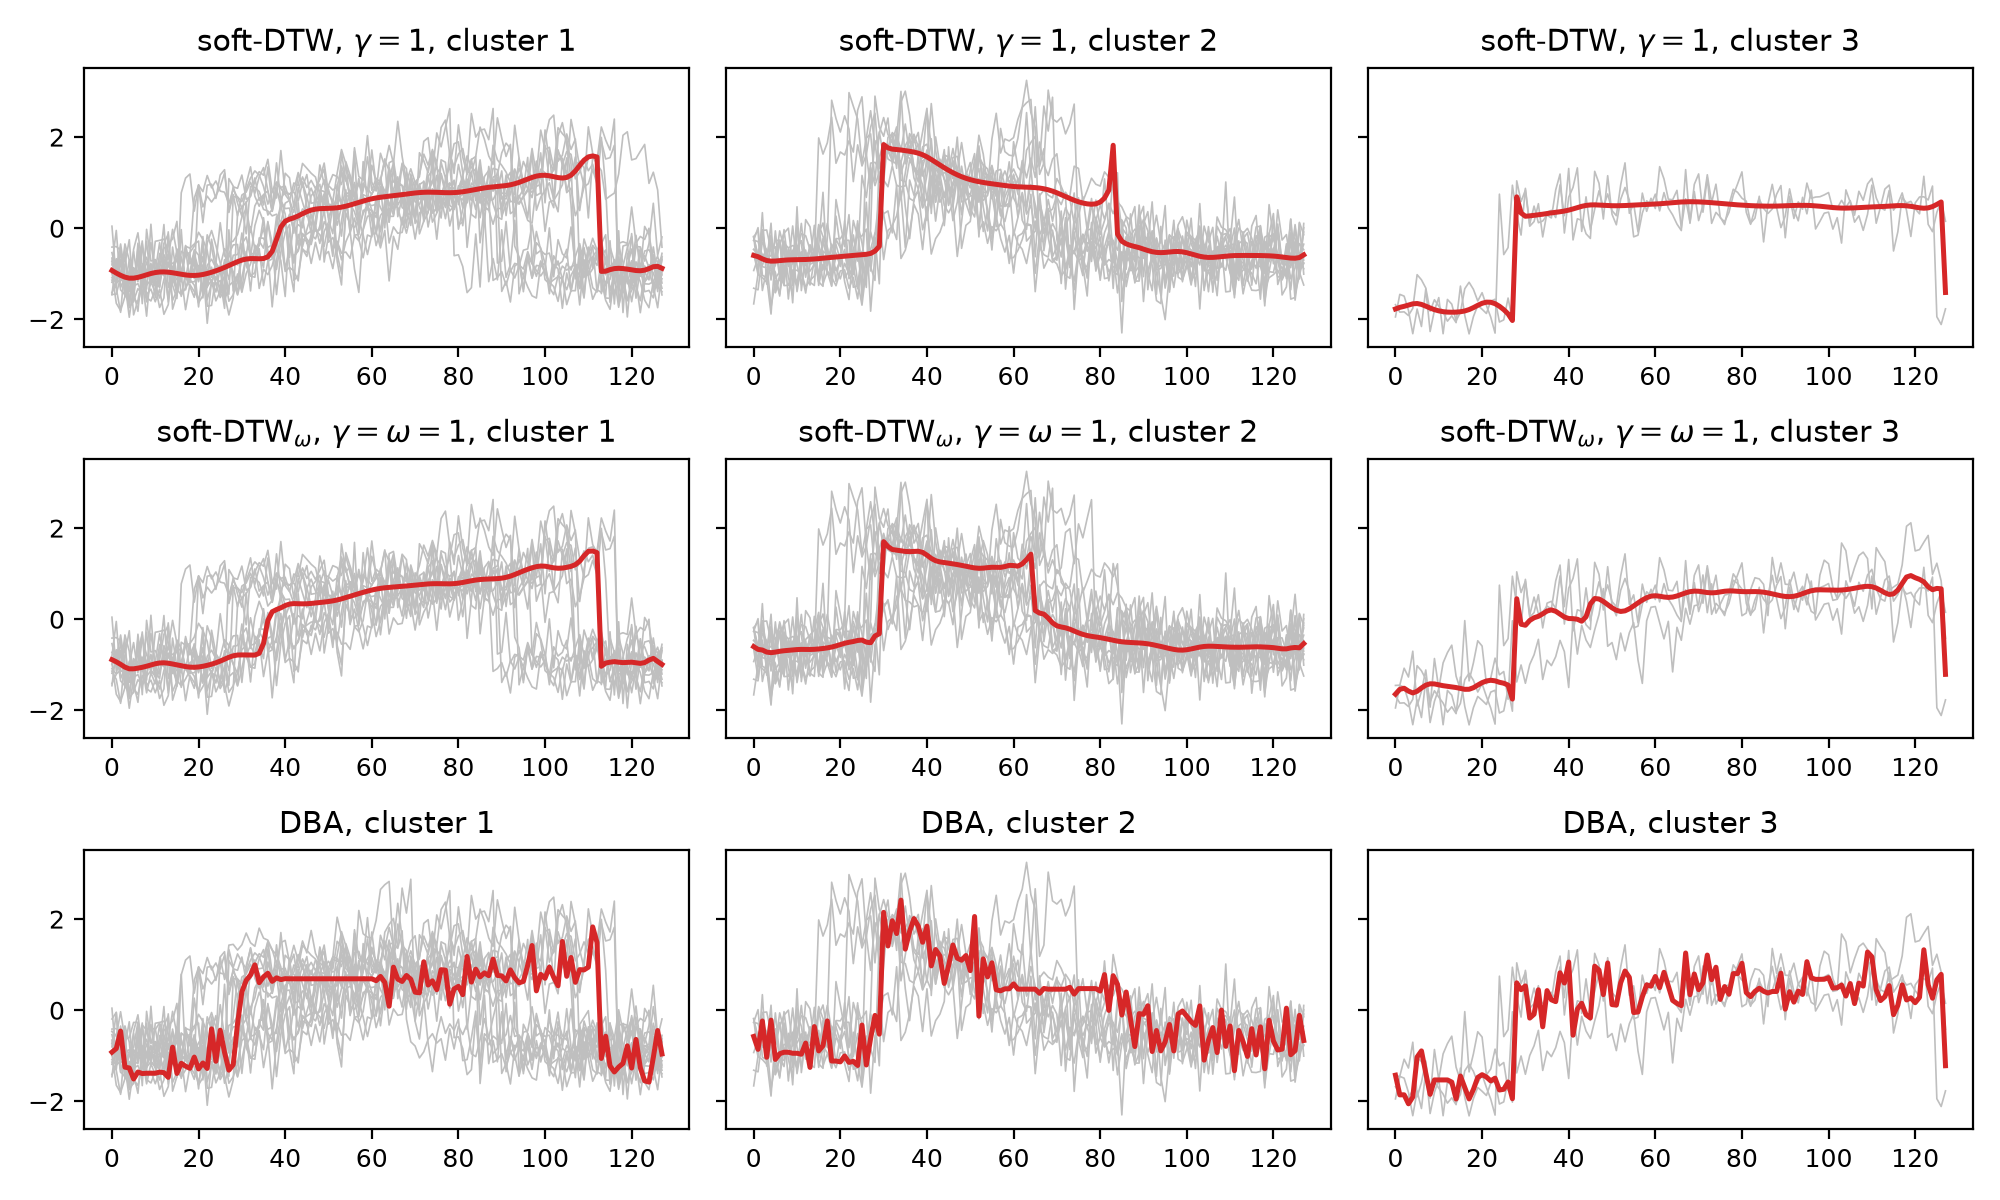
\includegraphics[width=\linewidth]{kmeans_CBF.png}
\caption{$k$-means clusters on CBF (paper's Fig.~6), same random initialisation. Soft-DTW and soft-DTW$_\omega$ ($\gamma=1$, $\omega=1$) centroids are smooth; DBA centroids absorb the noise of the series.}
\label{fig:kmeans}
\end{figure}

\begin{figure}[h]
\centering
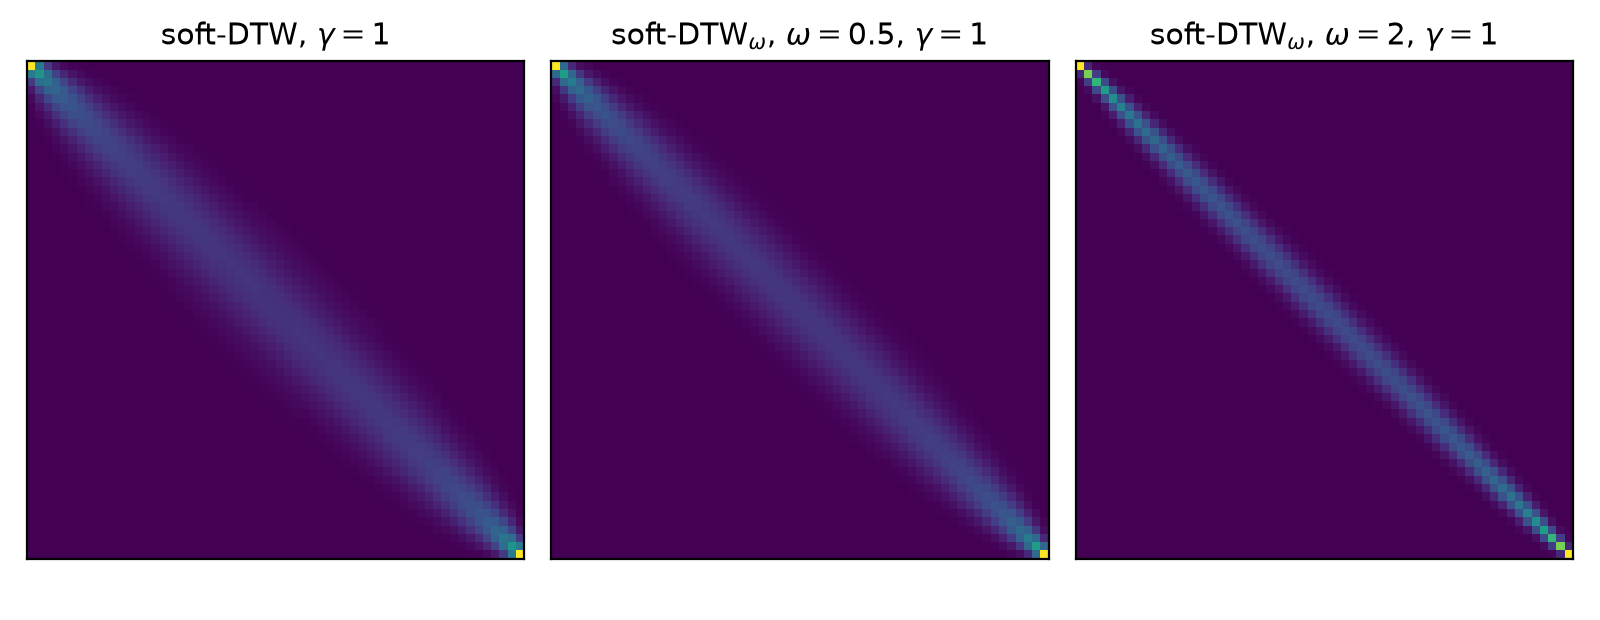
\includegraphics[width=0.7\linewidth]{prior_zero_cost.png}
\caption{Expected alignment $E$ between two identical constant series (all costs are zero), i.e.\ the data-independent prior of the soft-minimum over paths. Soft-DTW spreads it over a wide diagonal band; a warping penalty $\omega$ narrows it.}
\label{fig:prior}
\end{figure}


\end{document}
